\documentclass[12pt,a4paper]{article}
\usepackage[latin1]{inputenc}
\usepackage[brazil]{babel}
\usepackage{amsmath}
\usepackage{amsfonts}
\usepackage{amssymb}
\usepackage{graphicx}
\usepackage[top=2cm, bottom=2cm, left=3cm, right=2cm]{geometry}
\author{Leonardo Amorim - 15/0039921}
\title{\textbf{Teste 8 - Resolu��o usando if-then-else}}
\date{}
\begin{document}
\maketitle

Foi utilizado o exemplo do if-then-else.

\begin{figure}[!htb]
	\centering
	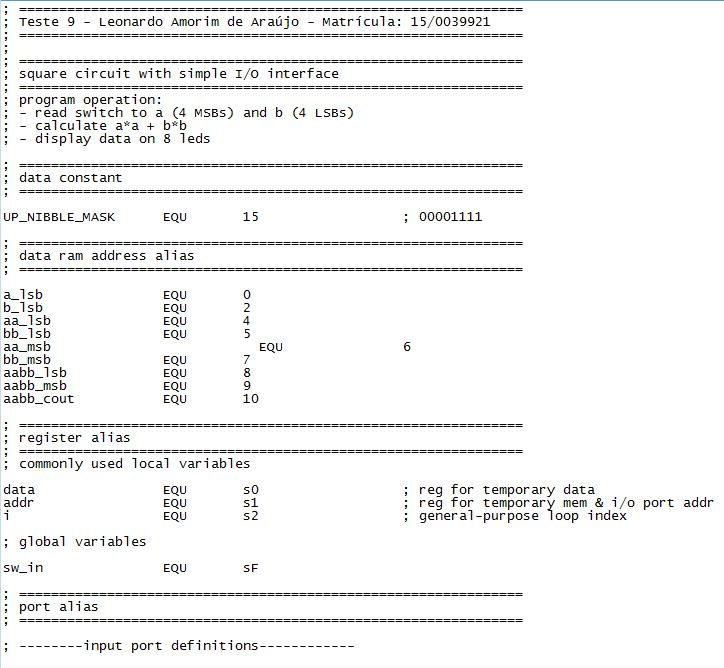
\includegraphics[scale=0.7]{codigo.jpg}
	\caption{C�digo utilizado}
\end{figure}

a) Abaixo segue uma amostra do funcionamento do c�digo.
\begin{figure}[!htb]
	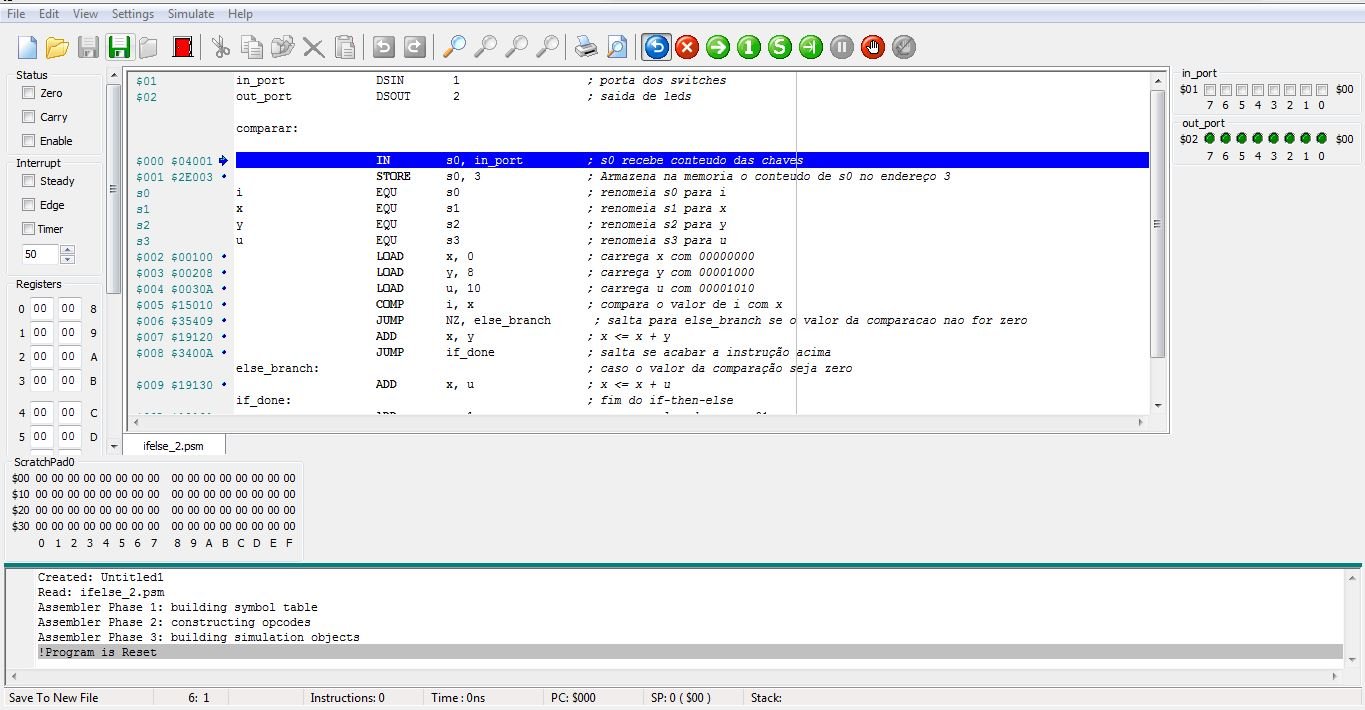
\includegraphics[scale=0.45]{simulacao.jpg}
	\caption{Simula��o do c�digo}
\end{figure}
\\
b) O codigo consiste em verificar se uma vari�vel i � ou n�o igual � zero. Duas constantes foram inseridas, uma chamada de y com um valor definido de 8 e outra chamada de u com um valor definido de 10. Outra constante, x � inicializada em 0. Caso i==0 , o valor de x � somado com y e depois acrescentado de 1, somado depois do if-then-else. Caso i=!0, o valor de x � somado com 10 e depois somado com um. Ap�s isto o valor � mostrado na sa�da (leds).

c) Abaixo vemos uma parte da simula��o do c�digo. Neste momento, os registradores j� foram carregados, o valor de i � diferente de zero, logo entrou-se na condi��o do else (realizou o jump) e vai ter o valor de x somado com 10.
\begin{figure}[!htb]
	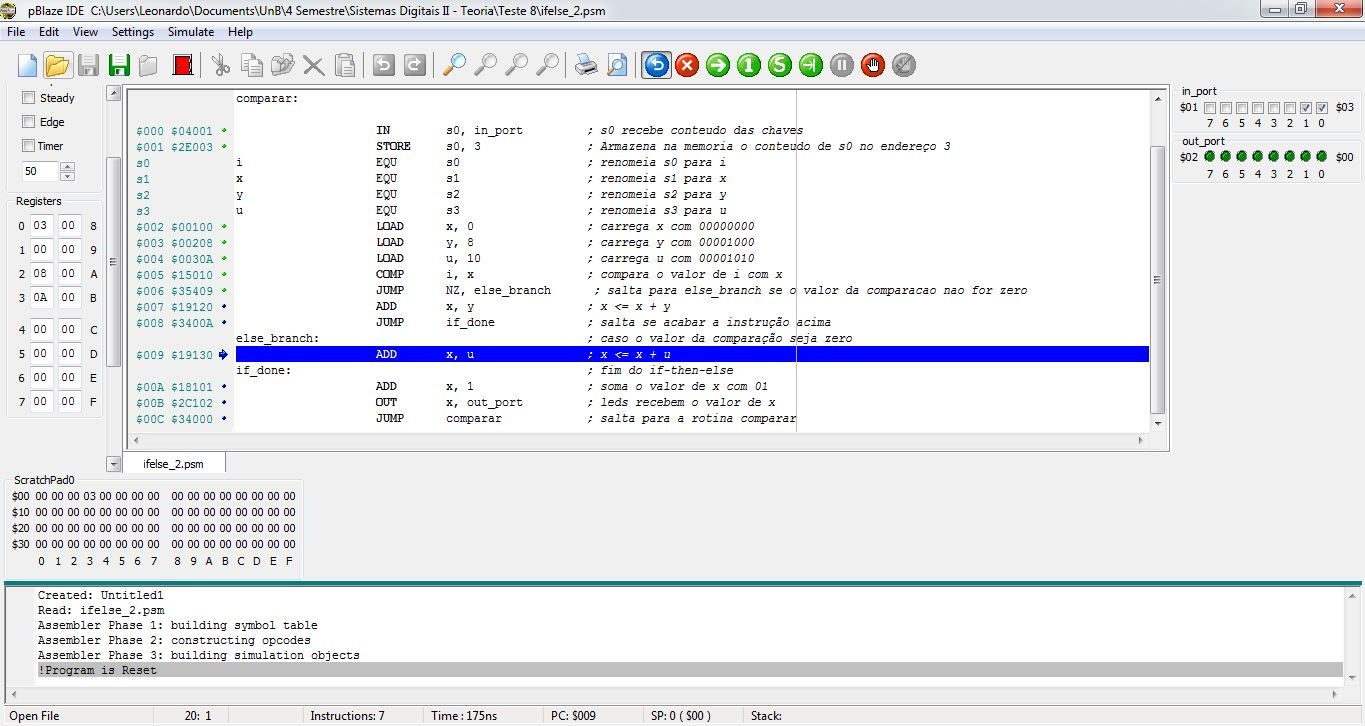
\includegraphics[scale=0.45]{simulacao1.jpg}
	\caption{Funcionamento}
	\label{simu}
\end{figure}
\\ d) Vemos ao t�rmino o valor novo na sa�da, conforme figura \ref{simu1}.
\begin{figure}[!htb]
	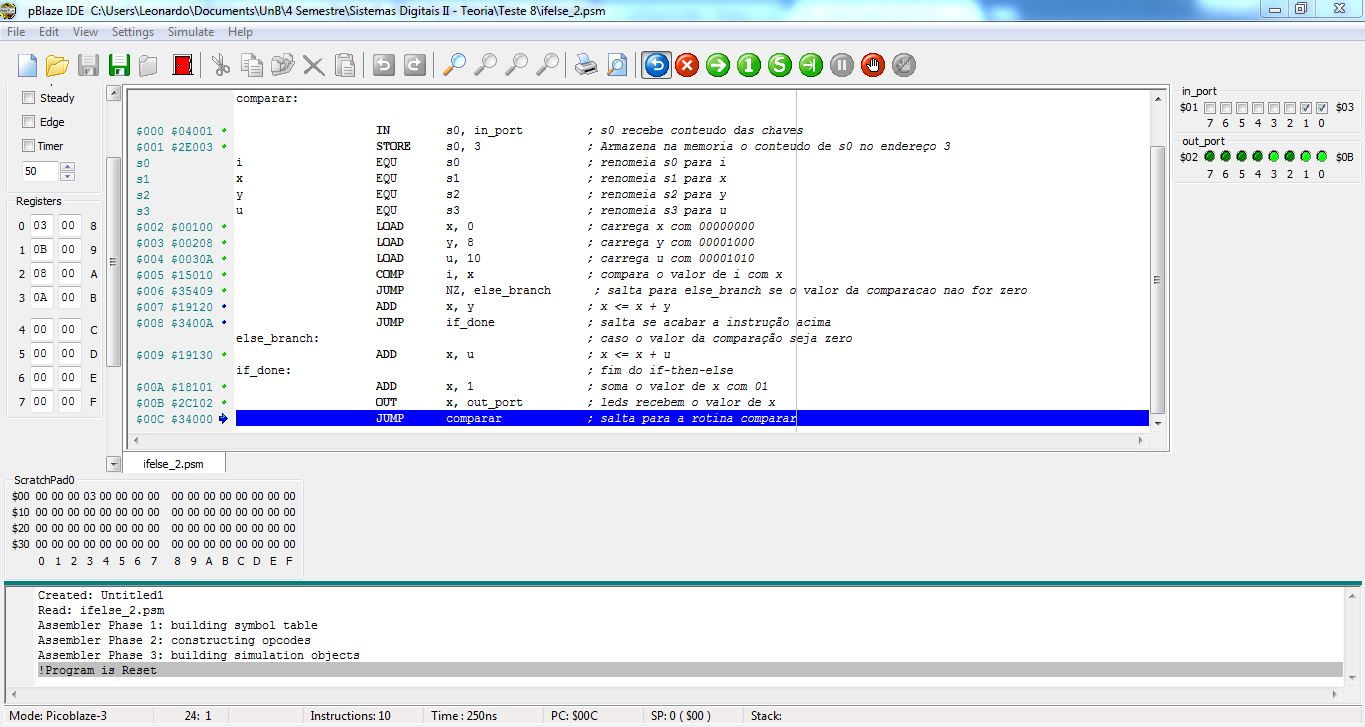
\includegraphics[scale=0.45]{simulacao2.jpg}
	\caption{Funcionamento ao t�rmino}
	\label{simu1}
\end{figure}
	
\end{document}